\documentclass[a4j]{jarticle}

\usepackage{graphicx}
\usepackage{url}
\usepackage{listings,jlisting}
\usepackage{ascmac}
\usepackage{amsmath,amssymb}

%ここからソースコードの表示に関する設定
\lstset{
  basicstyle={\ttfamily},
  identifierstyle={\small},
  commentstyle={\smallitshape},
  keywordstyle={\small\bfseries},
  ndkeywordstyle={\small},
  stringstyle={\small\ttfamily},
  frame={tb},
  breaklines=true,
  columns=[l]{fullflexible},
  numbers=left,
  xrightmargin=0zw,
  xleftmargin=3zw,
  numberstyle={\scriptsize},
  stepnumber=1,
  numbersep=1zw,
  lineskip=-0.5ex
}
%ここまでソースコードの表示に関する設定

\title{知能プログラミング演習II 課題0}
\author{グループ99\\
  2911XXXX 名工大輔\\
  {\small (グループレポートの場合は、グループ名および全員の学生番号と氏名が必要)}
}
\date{2019年10月7日}

\begin{document}
\maketitle

\paragraph{提出物} rep0
\paragraph{グループ} グループ99
\paragraph{メンバー}
\begin{tabular}{|c|c|c|}
  \hline
  学生番号&氏名&貢献度比率\\
  \hline\hline
  2911XXXX&名工大輔&25\\
  \hline
  2911YYYY&工大花子&30\\
  \hline
  2911ZZZZ&情報工介&20\\
  \hline
  2911UUUU&知能創太&25\\
  \hline
\end{tabular}



\section{課題の説明}
\begin{description}
\item[課題0-1] N番目のフィボナッチ数をもとめるプログラムを実装せよ.
\item[課題0-2] 自然界に現れるフィボナッチ数列の例を示し,なぜそれがフィボナッチ数列になるのかという原理を考察せよ.
\end{description}


\section{課題0-1}
\begin{screen}
  N番目のフィボナッチ数をもとめるプログラムを実装せよ.
\end{screen}

私の担当箇所は、後述するcalcFiboメソッドの実装である。
\subsection{手法}
課題に加えて、以下の3点を独自仕様として組み込んだ。

\begin{enumerate}
\item 与えられた数がフィボナッチ数かどうかを判定する。
\item N番目のフィボナッチ数だけではなく,N番目までのフィボナッチ数列を返す。
\item フィボナッチ数の一般項を用いてN番目のフィボナッチ数を求める。
\end{enumerate}

1.に関して、ユーザーから数字が与えられた時、それがフィボナッチ数である時に true を返し、フィボナッチ数ではない時には false を返す仕様とした。私はこのcalcFiboの実装を担当した。

2.に関しては、整数Nが与えられた時、0番目からN番目までのフィボナッチ数列を配列として返す仕様とした。

3.に関しては、・・・
\subsection{実装}

まず、プログラムに含まれるクラスは以下の1つ。
\begin{itemize}
\item Fibonacciクラス: メソッドcalcFibo, isFibo, calcFiboSeq, calcFiboGeneral を実装したクラス.Fibonacci.java に含まれる。
\end{itemize}

n番目のフィボナッチ数を計算するcalcFiboメソッドの実装をソースコード\ref{src:calcFibo}に示す。

\begin{lstlisting}[caption=calcFiboメソッド,label=src:calcFibo]
    // n番目のフィボナッチ数を計算して返す
    int calcFibo(int n) {
	if (n <= 1) {
	    return 1;
	}
	return calcFibo(n - 1) + calcFibo(n - 2);
    }
\end{lstlisting}

isFiboメソッドおよびcalcFiboSeqの実装については、グループレポートを参考にされたい。

calcFiboメソッドに渡す引数nをプログラム実行時に指定できるようにするため、mainメソッドおよびFibonacciクラスのコンストラクタを以下のように実装した。
\begin{lstlisting}[caption=mainメソッドとコンストラクタ,label=src:main]
    public static void main(String[] args) {
	new Fibonacci(Integer.parseInt(args[0]));
    }

    public Fibonacci(int n) {
	System.out.println(calcFibo(n));
    }
\end{lstlisting}

\subsection{実行例}
Fibonacciクラスに引数5を指定した実行結果を以下に示す。

\begin{lstlisting}
clf1XXXX@cse:~/eclipse-workspace/Fibo > java Fibonacci 5
8
\end{lstlisting}

今回は0, 1番目のフィボナッチ数を1としたため、calcFibo() の引数に5を与えた時は8となるのが正しい動作である。これは、・・・
\subsection{考察}
今回、フィボナッチ数をもとめるためのクラス Fibonacci を実装し、インスタンスメソッドとして機能を実装したが、これは静的クラスまたはシングルトンとして実装した方が適していたように考えられる。なぜなら・・・

また、calcFiboメソッドを再帰関数として実装するのではなく、イテレータを用いて実装した場合を考える。イテレータで実装した場合は、実行速度が・・・


\section{課題0-2}
\begin{screen}
  自然界に現れるフィボナッチ数列の例を示し,なぜそれがフィボナッチ数列になるのかという原理を考察せよ.
\end{screen}

課題0-2は実装を伴わない課題であるため、考察のみ記す。

\subsection{考察}
文献\cite{kijima2012}によると、ひまわりの種の並び方にフィボナッチ数列が隠れているという。具体的には、・・・。その原理は、・・・であると考えられる。何故なら、図\ref{fig:himawari} \cite{notty} に示すように、・・・

\begin{figure}[!hbt]
  \centering
  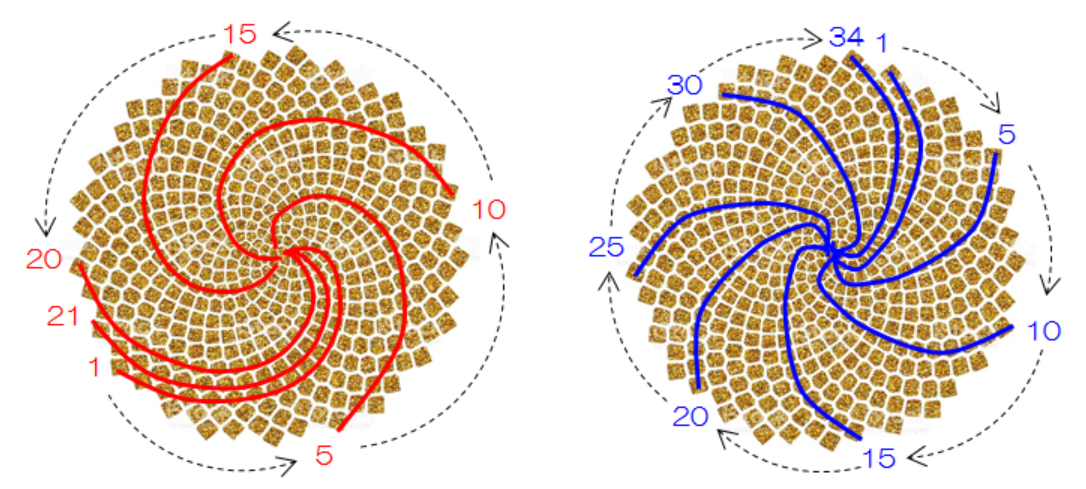
\includegraphics[bb=0 0 543 245,width=0.6\linewidth]{himawari.png}
  \caption{ひまわりの種の並び方\cite{notty}}
  \label{fig:himawari}
\end{figure}


\section{感想}
フィボナッチ数の一般項をもとめるのに夢中であやうく実装が間に合わなくなるところだった。実装に関しては、・・・


% 参考文献
\begin{thebibliography}{99}
\bibitem{kijima2012} 来嶋大二: ひまわりの螺旋, 数学のかんどころシリーズ 8, 共立出版, 2012.
\bibitem{notty} ひまわりに隠されたフィボナッチ数列と黄金比---ひまわりは黄金の花?, 数学の面白いこと・役に立つことをまとめたサイト, \url{https://analytics-notty.tech/fibonacci-and-goldenratio-in-sunflower/} (2019年10月4日アクセス).

\bibitem{hanako} 工大花子さんのレポート。また、・・・を教えてもらった 

\end{thebibliography}

\end{document}
